\section{Анализ предметной области. Постановка задачи}
\label{sec:domain}
 
В рамках данного раздела будет произведён обзор предметной области данного дипломного проекта.
Также будут рассмотрены возможные варианты реализаций и необходимые для этого технологий, сервисы, предлагающие аналогичные возможности, их плюсы и минусы и будут сформулированы основные требования к разрабатываемому ПО.
 
\subsection{Цель дипломного проекта}
Для определения ключевых функций приложения был произведён анализ статистики самых популярных и схожих по тематике приложений и сервисов. После изучения полученных результатов было решено, что необходимо создать современное приложение, которое совмещало бы в себе поиск приложений по популярным игровым магазинам, социальные функции, современный и простой интерфейс, который позволит пользователю в кратчайшие сроки найти себе приложение и магазин по душе.

\subsection{Формат разрабатываемого приложения}
В самом начале необходимо определиться с тем, как данное приложение будет функционировать. Под этим подразумевается необходимость выбора между разработкой настольного/мобильного или веб-приложения.
 
Под настольным приложением понимается программа, которую пользователь устанавливает на свой компьютер под управлением Windows/Linux, зачастую данные приложения требуют довольно долгой установки и зависимых библиотек уже установленных в системе.

Говоря о мобильном приложении, имеется в виду установочный файл/архив, который пользователь скачивает с магазина приложений. Для таких приложений система не требует дополнительных установок библиотек и работает всегда, за исключением критических ситуаций.

Веб-приложение довольно популярный формат в 2021 году и набирает популярность, не требует ничего кроме браузера, за исключением ситуаций, когда требуется определённая версия браузера.

Рассмотрим плюсы и минусы этих реализаций ПО.

Для настольных приложений характерна высокая степень интеграции с системой пользователя и более низкое потребление системных ресурсов, однако они стремительно теряют свою популярность, так как мобильные и веб-приложения оказываются в более выгодной ситуации в плане установки, потребления и простоте. Если говорить о ходе разработки настольных приложениях, то оно сопровождается множеством платформенных зависимостей, которые зачастую пропускают специфичные для ОС функции.

Разработка веб-приложения, которое позже нужно будет адаптировать под мобильные платформы, чаще всего совпадает с потерей UX пользователя, как такового. При переносе сайтов в мобильную среду теряются нативные функции платформ, которые делают использование приложений более приятным для пользователя. Так же это связано с потерей производтильности и оптимизацией ПО.

Рынок мобильных приложений растёт с каждой секундой огромными темпами, поэтому самый популярный и самый эффективный метод это разработка мобильных приложений под какие-либо сервисы. Каждый год Google выпускает новые версии своих SDK с новыми возможностями улучшить жизнь пользователя, что на 2021 год даёт огромное пространство для реализаций своих идей. На текущий момент выбрана реализация мобильного приложения для Android среды.

\subsection{Анализ аналогов}

\subsubsection{Game Deals Tracker}~\par
Мобильное приложение от компании J\&C Studio, предоставляющий пользователям поиска игр по таким магазинам как Steam и Playstation Store. Game Deals Tracker обладает сравнительно небольшим функционалом: поиск, отображение скидок, вкладка "Рекомендуемые", возможность фильтровать результаты. Из важных для проекта возможностей стоит выделить, функцию просмотра скриншотов игр из Steam и Playstation Store, а так же просмотром отзывов из этих магазнов. На рисунке~\ref{fig:domain:game_deals_tracker} можно видеть пример отображения информации об игре из Steam. Так же хорошей функцией является вкладка "Исследовать" , которая является своеобразным дашбордом, в который пользователь может заходить без конкретной цели и искать себе игры по душе.
 
\begin{figure}[H]
 \centering
   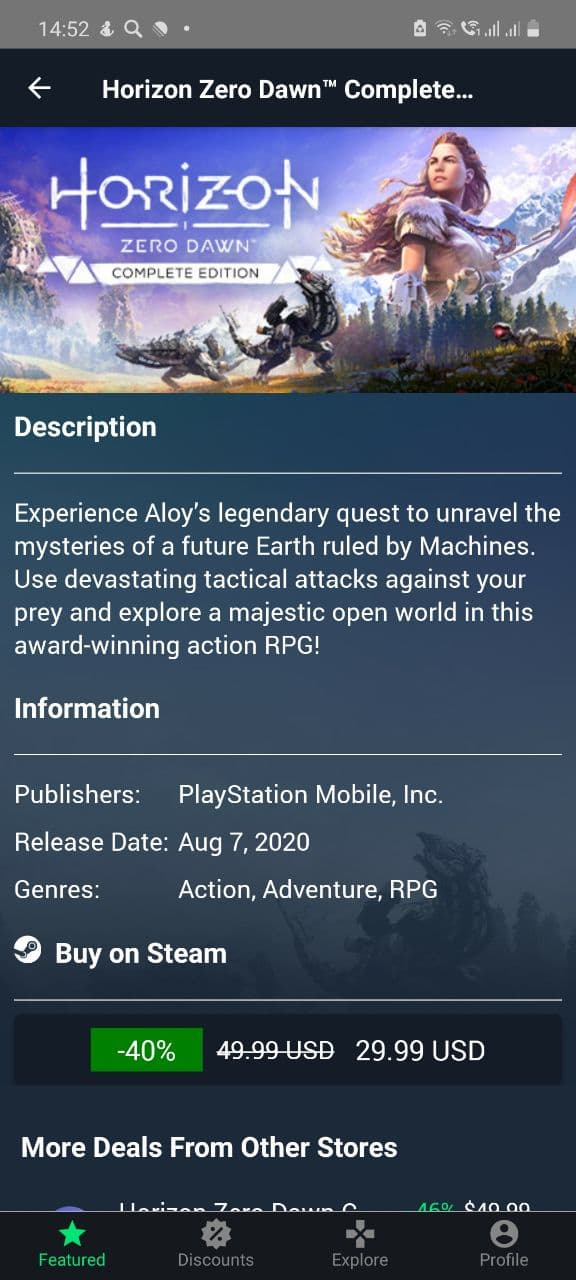
\includegraphics[scale=0.4]{game_deals_tracker.jpg} 
   \caption{Отдельная игра из Steam}
   \label{fig:domain:game_deals_tracker}
\end{figure}
 
Плюсы:
\begin{itemize}
 \item неплохой UI/UX;
 \item вкладка "Исследовать";
 \item отображение отзывов и скриншотов из Steam;
 \item возможность синхронизировать настройки через единый аккаунт;
 \item поиск и его фильтры.
\end{itemize}
 
Минусы:
\begin{itemize}
 \item в основной части приложения всего два магазина для основного поиска и работы с его результатами;
 \item для вкладки с сохранением понравившихся предложений и игр пользователь обязан регистрироваться;
 \item реклама при переходах на отдельные экраны.
\end{itemize}
 
\subsubsection{Bargain Bytes - Game Deals}~\par
Game Deals от Rockspin, довольно популярное приложение, обладающие простым функционалом по поиску игр из разных магазинов. Главными функциями данного приложения является поиск по множеству магазинов, а так же удобная вкладка WatchList, которая присылает нотификации в центр уведомлений телефона, когда цена упала до определённой отметки, что зачастую является очень удобной функцией для конечного пользователя. (пример на рисунке~\ref{fig:domain:game_deals_bytes}).
 
\begin{figure}[H]
 \centering
   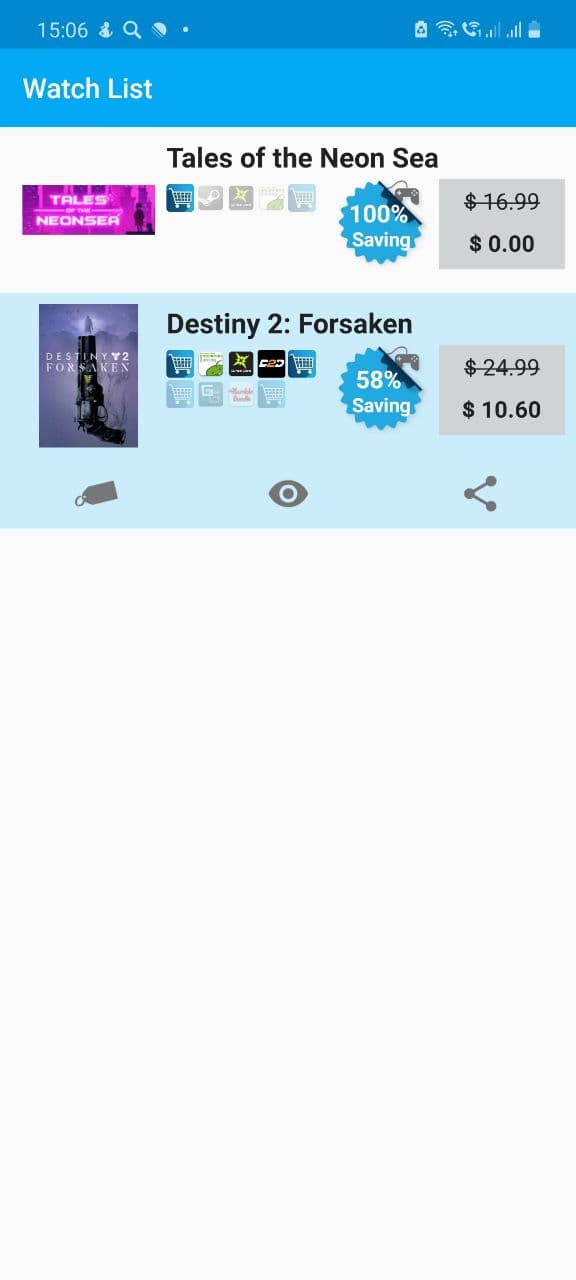
\includegraphics[scale=0.4]{game_deals_bytes.jpg} 
   \caption{Вкладка WatchList}
   \label{fig:domain:game_deals_bytes}
\end{figure}
 
Плюсы:
\begin{itemize}
 \item простой интерфейс;
 \item не требуется регистрация;
 \item множество магазинов.
\end{itemize}
 
Минусы:
\begin{itemize}
 \item устаревший UI/UX;
 \item приложение неоптимизированно;
 \item мало информации о конкретном предложении.
\end{itemize}

\subsubsection{CheapShark.com}~\par
CheapShark.com от AngrySoftware. Удобное настольное приложение для Windows, позволяет искать по разным магазинам и находить нужное приложение. Из отличительных функций нотификации на емейл по конкретному предложению, когда цена достигнет нужной отметки. Неплохим функционалом является просмотр игр от конкретного магазина. (пример на рисунке~\ref{fig:domain:game_cheap_shark}).

\begin{figure}[H]
  \centering
    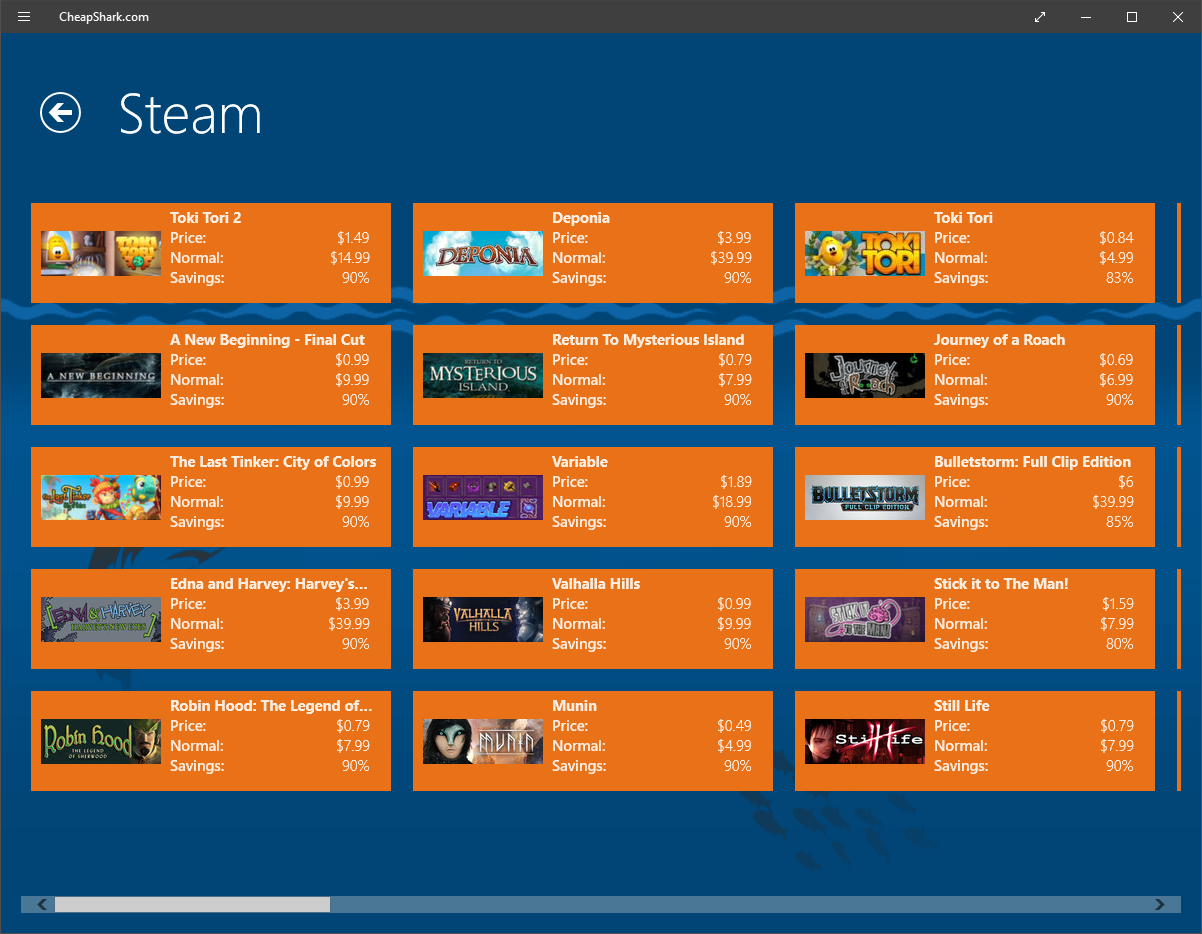
\includegraphics[scale=0.5]{game_deals_cheap_shark.png} 
    \caption{Приложение CheapShark}
    \label{fig:domain:game_cheap_shark}
 \end{figure}

Плюсы:
\begin{itemize}
  \item удобный настольный интерфейс;
  \item множество магазинов;
  \item просмотр игр по отдельному магазину;
  \item отсутствует реклама.
\end{itemize}

 Минусы:
 \begin{itemize}
  \item очень мало функционала;
  \item нет поиска;
  \item показаны не все игры от магазина;
  \item нет фильтров.
\end{itemize}
 
\subsection{Постановка задачи}
В рамках данного дипломного проекта необходимо разработать мобильное приложение агрегатор игровых магазинов. При разработке необходимо выполнить следующие задачи:
\begin{itemize}
 \item разработать приложение, которое будет агрегировать игровые магазины;
 \item разработать пользовательский интерфейс для приложения;
 \item реализовать поддержку сторонних ресурсов: Steam, Metacritic, и так далее.
\end{itemize}
 
\subsection{Требования к приложению}
Одним из самых важных этапов при разработке является сбор и организация требований. Хорошо описанные требования существенно снижают риски при проектировании архитектуры, разработке и тестировании программного продукта.
 
\subsubsection{Нефункциональные требования}
\begin{itemize}
 \item минимизировать затраты на разработку первой версии приложения;
 \item мобильное приложение должно работать на большом количестве мобильных устройств, минимальная версия Android SDK 23+;
 \item поддержка новейшего Android API;
 \item сопровождение более старых версий Android.
\end{itemize}
 
\subsubsection{Функциональные требования}
\begin{itemize}
  \item поддержка множества магазинов;
  \item возможность фильтровать ответы;
  \item вкладка избранное;
  \item вкладка исследование;
  \item возможность удобного поиска.
  % \item плеер имеет текстовый чат;
\end{itemize}
 
\subsection{Перспективы развития приложения}
В дальнейшем приложение может быть улучшено при помощи введения дополнительных возможностей:
\begin{itemize}
  \item подключение дополнительных функций для разных магазинов;
  \item собственная библиотека игр;
  \item инетграция прямых трансляций по определенной игре;
  \item расширение списка магазинов;
  \item добавление большего числа социальных функций.
\end{itemize}
